\documentclass[a4paper, 14pt]{extarticle}

\usepackage[T2A]{fontenc}
\usepackage{natbib}
\usepackage{graphicx}
\usepackage[english, russian]{babel}
\usepackage{fontspec}
\usepackage{amsmath}
\usepackage{amsfonts}
\usepackage{amssymb}
\usepackage{amsthm}
\usepackage{mathtools}
\usepackage{mathrsfs}
\usepackage{icomma}
\usepackage{fullpage}
\usepackage{ulem}
\usepackage{setspace}
\usepackage{listings}
\usepackage{indentfirst}
\usepackage[left=2cm,right=1.5cm,top=2cm,bottom=2cm]{geometry}
\usepackage{xcolor}
\usepackage{float}
\usepackage{csquotes}
\usepackage{hyperref}
\usepackage{graphics}



\definecolor{urlcolor}{HTML}{0000FF} % цвет гиперссылок
\definecolor{linkcolor}{HTML}{000000} % цвет гиперссылок
\hypersetup{pdfstartview=FitH, linkcolor=linkcolor, urlcolor=urlcolor, colorlinks=true}


\setmainfont{Times New Roman}
\setlength{\parindent}{5ex}
\setlength{\parskip}{1em}
\renewcommand{\baselinestretch}{1}

\graphicspath{{images/}}


\definecolor{buzzlightyear}{HTML}{8757A5}
\definecolor{grass}{HTML}{738D06}
\definecolor{literal}{HTML}{F18A2B}
\definecolor{commentcolor}{HTML}{8E908B}

\lstdefinestyle{habrstyle}{
    backgroundcolor=\color{white},
    commentstyle=\color{commentcolor},
    keywordstyle=\bfseries\color{buzzlightyear},
    numberstyle=\tiny\color{commentcolor},
    stringstyle=\color{grass},
    basicstyle=\ttfamily\footnotesize,
    breakatwhitespace=false,
    breaklines=true,
    captionpos=b,
    keepspaces=true,
    numbers=left,
    numbersep=5pt,
    showspaces=false,
    showstringspaces=false,
    showtabs=false,
    tabsize=4
}

\lstset{style=habrstyle}

\begin{document}
    % НАЧАЛО ТИТУЛЬНОГО ЛИСТА
    \begin{center}
        \begin{center}
            \hfill \break
            \normalsize{Санкт-Петербургский государственный политехнический}\\
            \normalsize{университет Петра Великого}\\
            \hfill \break
            \normalsize{\textbf{Высшая школа интеллектуальных систем и}}\\
            \normalsize{\textbf{суперкомпьютерных технологий}}\\
            \hfill \break
            \hfill \break
            \hfill \break
            \normalsize{Лабораторная работа}\\
            \hfill \break
            \normalsize{\LARGE Линейные стационарные системы}\\
        \end{center}
        \hfill \break
        \hfill \break
        \hfill \break
        \hfill \break
        \hfill \break
        \hfill \break
        \hfill \break
        \hfill \break
        \hfill \break
        \hfill \break
        \begin{tabbing}
            Выполнил студент гр. 3530901/80201 \`И.С. Иванов\\
            \\
            Преподаватель: \`Н.В. Богач\\
        \end{tabbing}
        \hfill \break
        \hfill \break
        \hfill \break
        \hfill \break
        \begin{center}
            Санкт-Петербург\\
            2021
        \end{center}
        \thispagestyle{empty}
    \end{center}
    % КОНЕЦ ТИТУЛЬНОГО ЛИСТА

    % ОГЛАВЛЕНИЕ
    \newpage
    \tableofcontents

    % СПИСОК ИЛЛЮСТРАЦИЙ
    \newpage
    \listoffigures

    % СПИСОК ЛИСТИНГОВ
    \newpage
    \lstlistoflistings

    \newpage


    \section{Упражнение №1}
    \label{sec:1}

    В первом упражнении необходимо просмотреть примеры из файла \texttt{chap10.ipynb}.
    Далее изменить пример, чтобы устранить лишнюю ноту в начале фрагмента.

    Начнем с звука выстрела.

    \begin{lstlisting}[language=Python, caption= Считывание и обработка сигнала, label={lst:read_wave_gunshot}]
        from thinkdsp import read_wave

        response = read_wave('Sounds/180960__kleeb__gunshot.wav')

        start = 0.12
        response = response.segment(start=start)
        response.shift(-start)

        response.truncate(2**16)
        response.zero_pad(2**17)

        response.normalize()
        response.plot()
        decorate(xlabel='Time (s)')
    \end{lstlisting}

    \begin{figure}[H]
        \centering
        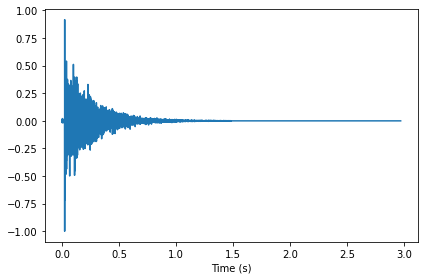
\includegraphics[width=0.8\linewidth]{gunshot_wave}
        \caption{Сигнал выстрела}
        \label{fig:gunshot_wave}
    \end{figure}

    Построим спектр.

    \begin{figure}[H]
        \centering
        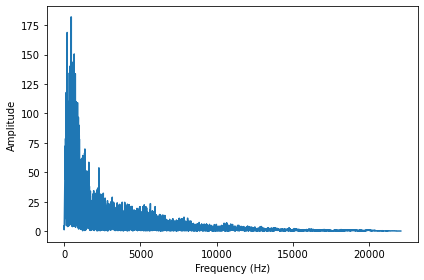
\includegraphics[width=0.8\linewidth]{gunshot_spectrum}
        \caption{Спектр сигнала выстрела}
        \label{fig:gunshot_spectrum}
    \end{figure}

    Теперь возьмем звук скрипки и проделаем тоже самое.

    \begin{figure}[H]
        \centering
        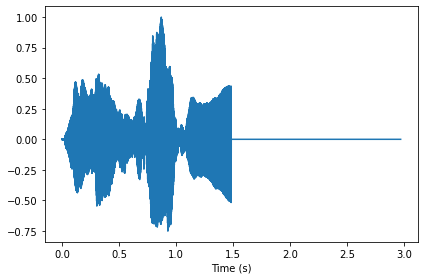
\includegraphics[width=0.8\linewidth]{violin_wave}
        \caption{Сигнал скрипки}
        \label{fig:signal_cumsum}
    \end{figure}

    После умножим ДПФ сигнала на передаточную функцию, преобразуем обратно в сигнал и выведем на экран.

    \begin{figure}[H]
        \centering
        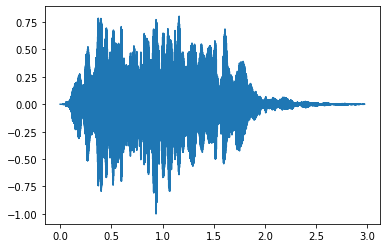
\includegraphics[width=0.8\linewidth]{violin_spectrum}
        \caption{Сигнал после обработки}
        \label{fig:violin_spectrum}
    \end{figure}

    При прослушивании получившегося сигнала можно сделать вывод, что "затекшей" ноты в начале больше нет.

    \newpage


    \section{Упражнение №2}
    \label{sec:2}

    В втором упражнении необходимо смоделировать двумя способами звучание записи в том пространстве, где была измерена импульсная характеристика, как сверткой замой записи с импульсной характеристикой, так и умножением ДПФ записи на вычислительный фильтр.

    Считаем импульсную характеристику из библиотеки \texttt{OpenAir}.
    Окружение Central Hall, University of York.

    \begin{lstlisting}[language=Python, caption= Считывание импульсной характеристики, label={lst:read_ir}]
        response = read_wave('Sounds/ir_row_1l_sl_centre.wav')

        start = 0
        response.shift(-start)

        response.normalize()
        response.plot()
        decorate(xlabel='Time (s)')
    \end{lstlisting}

    \begin{figure}[H]
        \centering
        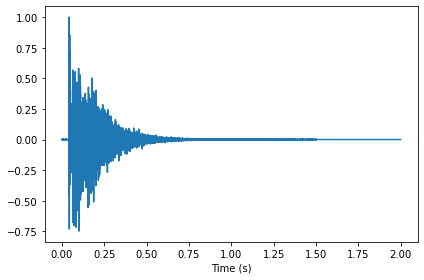
\includegraphics[width=0.8\linewidth]{ir_wave}
        \caption{Полученный сигнал}
        \label{fig:ir_wave}
    \end{figure}

    Получим спектр сигнала.

    \begin{figure}[H]
        \centering
        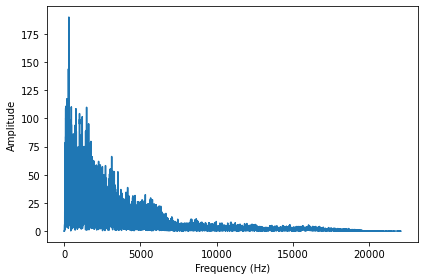
\includegraphics[width=0.8\linewidth]{ir_spectrum}
        \caption{Спектр сигнала}
        \label{fig:ir_spectrum}
    \end{figure}

    Посмотрим на спектр в логарифмическом масштабе.

    \begin{figure}[H]
        \centering
        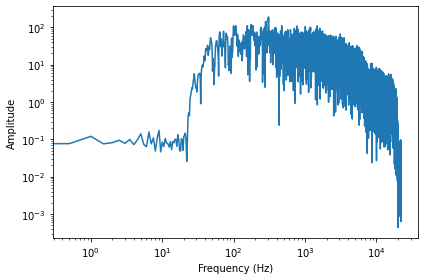
\includegraphics[width=0.8\linewidth]{ir_spectrum_log}
        \caption{Логарифмический спектр}
        \label{fig:ir_spectrum_log}
    \end{figure}

    Смоделируем звучание записи, под нахождение в комнате записи импульсной характеристики.

    Считаем файл и посмотрим его график.

    \begin{figure}[H]
        \centering
        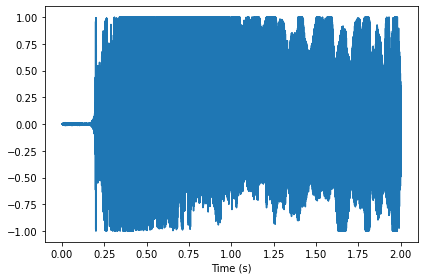
\includegraphics[width=0.8\linewidth]{scream_wave}
        \caption{Сигнал записи}
        \label{fig:scream_wave}
    \end{figure}

    Также была обрезана запись звука до длины импульсной характеристики.

    Выполним умножение в частотной области и преобразуем обратно во временную.
    Выведем результат.

    \begin{figure}[H]
        \centering
        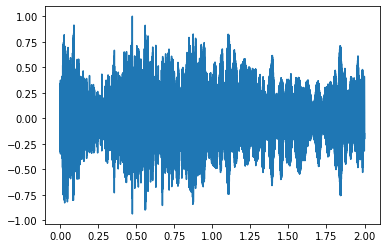
\includegraphics[width=0.8\linewidth]{scream_result}
        \caption{Результат}
        \label{fig:scream_result}
    \end{figure}

    Представим полученный сигнал в виде аудио.
    Далее воспользуемся методом \texttt{convolve} для свертки.

    В результате выполнения был получен звук играющий в помещении импульсной характеристики.

    \newpage


    \section{Выводы}
    \label{sec:conclusions}

    В результате выполнения данной лабораторной работы были получены знания о свертке сигналов.
    Была модифицирована запись игры на скрипке, в которой была убрана первая нота.
    Также было произведено моделирование звучание записи в помещении.

\end{document}